\twocolumn[{%
\renewcommand\twocolumn[1][]{#1}%
\noindent\begin{minipage}{\linewidth} 
 	\begin{center}
 	\vspace{0.3cm}
 	\captionsetup{font=small}
 	\begin{tabular}{@{}c@{}c@{}c@{}c@{}}
 	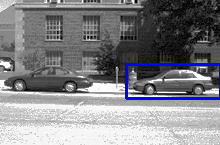
\includegraphics[width=0.24\linewidth]{fig6_a1} &
	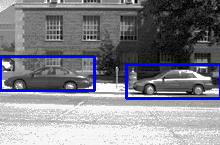
\includegraphics[width=0.24\linewidth]{fig6_b1} &
 	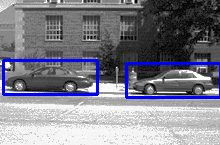
\includegraphics[width=0.24\linewidth]{fig6_c1} &
 	 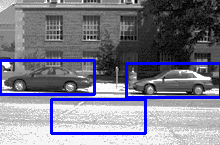
\includegraphics[width=0.24\linewidth]{fig6_d1} \vspace{-1mm}\\ 
 	 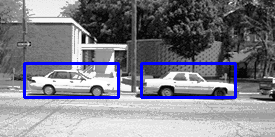
\includegraphics[width=0.24\linewidth]{fig6_a2} &
	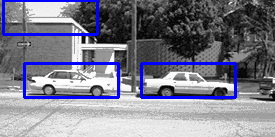
\includegraphics[width=0.24\linewidth]{fig6_b2} &
	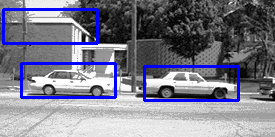
\includegraphics[width=0.24\linewidth]{fig6_c2} &
 	 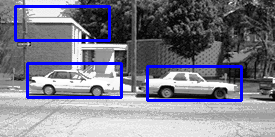
\includegraphics[width=0.24\linewidth]{fig6_d2} \vspace{-1mm}\\   
    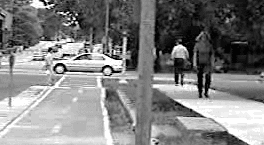
\includegraphics[width=0.24\linewidth]{fig6_a3} &
	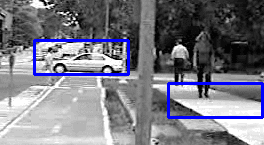
\includegraphics[width=0.24\linewidth]{fig6_b3} &
 	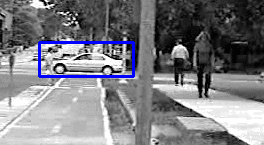
\includegraphics[width=0.24\linewidth]{fig6_c3} &
 	 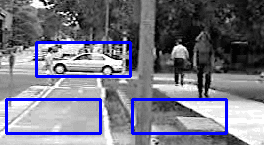
\includegraphics[width=0.24\linewidth]{fig6_d3}  \vspace{-1mm}\\
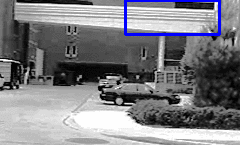
\includegraphics[width=0.24\linewidth]{fig6_a4} &
	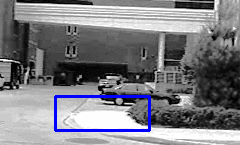
\includegraphics[width=0.24\linewidth]{fig6_b4} &
 	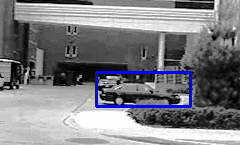
\includegraphics[width=0.24\linewidth]{fig6_c4} &
 	 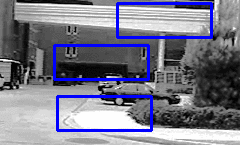
\includegraphics[width=0.24\linewidth]{fig6_d4} \vspace{-1mm}\\

    {\small (a)} &  {\small (b)}  &  {\small (c)} &  {\small (d)} \\
    \end{tabular}
	\captionof{figure}{\small 不同分类器在车辆侧视数据集上的检测结果。(a) Logistic 回归, (b) 支持向量机, (c) AdaBoost, and (d) AdaBoost$^*$.}
	\label{fig:result}
	\end{center}
	\vspace{0.5cm}
\end{minipage}
}]

\section{实验}
\label{sec:experiment}


这一章节将会利用上一章介绍的高斯混合模型的背景建模方法在视频序列图像上进行实验,并对其实现效果、实时性进行展示和分析。

\subsection{数据集}

传统的基于滑窗的目标检测算法将在静态场景下的侧视车辆数据集上进行实验,其中训练集包含 550 个正例样本和 500 个负例样本,共有 170 张测试图片。利用 sklearn 中的 train\_test\_split 方法按照 4:1 对数据集进行训练集和验证集的划分。划分好数据集后,利用 HOG 对训练集数据的图片进行特征提取并对 PCA 降维模型进行训练,将 27104 维数据降维至 300 维。

基于深度学习的口罩检测将在 Mask Wearing 数据集上进行实验,数据集包含用于训练模型的图像 468 张、用于模型验证的图像 116张和用于模型性能测试的图像 95 张。图像的标签以 xml 格式标注,标注文件中包含目标的类别(good:佩戴口罩,bad:未佩戴口 罩,none:未正确佩戴口罩)及其边界框左上角和右下角的(x,y)坐标值。

\subsection{评价指标}

选择 Recall、Precision 和 F-measure 指标对模型结果进行评测。在介绍这三个指标前需要明确四个概念:TP、FP、TN、FN。


\begin{table}[htbp]
  \centering
  \caption{分类结果混淆矩阵}
  \setlength{\tabcolsep}{7mm}{
    \begin{tabular}{c|c|c}
    \toprule
    \multirow{2}[4]{*}{真实情况} & \multicolumn{2}{c}{预测结果} \\
\cmidrule{2-3}          & 正例    & 反例 \\
    \midrule
    正例    & TP(真正例) & FN(假反例) \\
    \midrule
    反例    & FP(假正例) & TN(真反例) \\
    \bottomrule
    \end{tabular}%
  \label{tab:matrixl}}
\end{table}%


Recall、Precision 和 F-measure 相应的计算方法如下: 

\begin{equation}
\begin{aligned}
	查全率(precision) &= \frac{TP}{TP+FP}\\
	查准率(recall) &= \frac{TP}{TP+FN}
\end{aligned}
\end{equation}

查全率和查准率是一对矛盾的度量,一般来说,查准率高时,查全率往往偏低;而查全率高时,查准率往往偏低。通常只有在一些简单任务中,才可能使查全率和查准率都很高。在两者都要求高的情况下,综合衡量查全率和查准率就用 F1 值,其计算方法如下:

\begin{equation}
	F1 = \frac{2\times precision \times recall}{precision + recall}
\end{equation}

\subsection{车辆检测}

不同分类器的训练结果如表 \ref{tab:class_result} 所示,其中 AdaBoost$^*$ 表示采用参数 algorithm='SAMME.R', learning\_rate=1.0, n\_estimators=100, random\_state=0 训练得到的分类器。测试时,利用与训练图片等大的窗口大小对待检测图片进行滑窗。然后对每个窗进行分类,判断其是否为汽车。如果是汽车则将其保存为候选,最后利用所有候选带入 NMS 算法计算得到最终的检测框。由于测试集未给出标签,统计结果如表 \ref{tab:count} 所示,计算指标如表 \ref{tab:metric}所示,部分检测结果如图 \ref{fig:result} 所示。

\begin{table*}[!ht]
	\centering
	\caption{分类器训练测试结果表}
	\begin{subtable}[t]{0.495\linewidth}
	\caption{Logistic 回归}
	\begin{tabular}{c|cccc}
		\toprule
		& Precision&Recall & F1 Score &Support\\\hline
		no car&1.00&0.97&0.99&109\\
		car &0.97&1.00&0.99&101\\\hline
		accuracy&&&0.99&210\\ 
		macro average &0.99&0.99&0.99&210\\
		weighted avg&0.99&0.99&0.99&210\\
		\bottomrule
	\end{tabular}
	\end{subtable}
	\begin{subtable}[t]{0.495\linewidth}
	\caption{支持向量机}
	\begin{tabular}{c|cccc}
		\toprule
		& Precision&Recall & F1 Score &Support\\\hline
		no car&0.99&1.00&1.00&105\\
		car &1.00&0.99&1.00&105\\\hline
		accuracy&&&1.00&210\\ 
		macro average &1.00&1.00&1.00&210\\
		weighted avg&1.00&1.00&1.00&210\\
		\bottomrule
	\end{tabular}
	\end{subtable}

	\begin{subtable}[t]{0.495\linewidth}
	\caption{AdaBoost}
	\begin{tabular}{c|cccc}
		\toprule
		& Precision&Recall & F1 Score &Support\\\hline
		no car&1.00&0.96&0.98&102\\
		car &0.96&1.00&0.98&108\\\hline
		accuracy&&&0.98&210\\ 
		macro average &0.98&0.98&0.98&210\\
		weighted avg&0.98&0.98&0.98&210\\
		\bottomrule
	\end{tabular}
	\end{subtable}
	\begin{subtable}[t]{0.495\linewidth}
	\caption{AdaBoost$^*$}
		\begin{tabular}{c|cccc}
		\toprule
		& Precision&Recall & F1 Score &Support\\\hline
		no car&1.00&1.00&1.00&109\\
		car &1.00&1.00&1.00&101\\\hline
		accuracy&&&1.00&210\\ 
		macro average &1.00&1.00&1.00&210\\
		weighted avg&1.00&1.00&1.00&210\\
		\bottomrule
	\end{tabular}
	\end{subtable}
	\label{tab:class_result}
\end{table*}

\begin{table}[!ht]
\centering
\caption{不同分类器的检测结果}
\setlength{\tabcolsep}{6mm}{
\begin{tabular}{c|c|c|c}
	\toprule
	分类器&TP&FP&FN\\\hline
	Logistic 回归 & 183&5&19\\
	支持向量机&196&36&6\\
	AdaBoost&198&54&4\\
	AdaBoost$^*$&198&80&4\\
	\bottomrule
\end{tabular}}
\label{tab:count}
\end{table}

\begin{table}[!ht]
\centering
\caption{不同分类器的指标}
\setlength{\tabcolsep}{4mm}{
\begin{tabular}{c|c|c|c}
	\toprule
	分类器&Precision&Recall&F1 Score\\\hline
	Logistic 回归 & 0.97&0.91&0.94\\
	支持向量机&0.84&0.97&0.90\\
	AdaBoost&0.79&0.98&0.83\\
	AdaBoost$^*$&0.71&0.98&0.82\\
	\bottomrule
\end{tabular}}
\label{tab:metric}
\end{table}

综合来看,虽然支持向量机和 AdaBoost 方法检测的真正例(TP)更多,但从其他指标及可视化检测结果可以看出,其查全率的提升是以查准率为代价的,如图 \ref{fig:result} (d) 所示,虽然 AdaBoost 检测出的真正例更多,查全率较高,但是其检测出的假正例也相对更多,导致模型的查准率下降。在一定程度上可以认为是模型过拟合造成的,即过度拟合训练数据的特征,误把训练数据中的噪声也认为是车辆特征进行了学习。同时也反映出查全率和查准率难以同时达到很高。

不同分类器的实时性分析如表 \ref{tab:time} 所示。

\begin{table}[!ht]
\centering
\caption{不同分类器的实时性比较}
\setlength{\tabcolsep}{1mm}{
\label{time}
\begin{tabular}{c|c|c|c|c}
\toprule
&Logistic 回归& SVM &AdaBoost&AdaBoost$^*$\\\hline
单张耗时(秒)&9.508&6.019&42.11&53.56\\
\bottomrule	
\end{tabular}}
\label{tab:time}
\end{table}

\subsection{基于深度学习的口罩检测}

\begin{figure}[!ht]
	\centering
	\begin{minipage}[t]{0.235\linewidth}
		\centering
		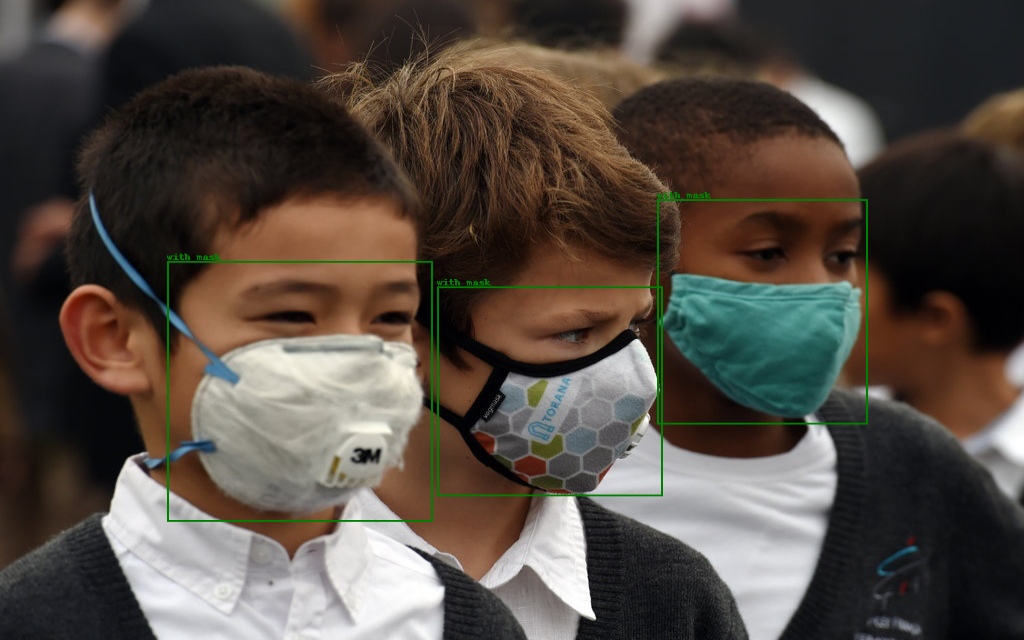
\includegraphics[width=\linewidth]{fig7a.png}\\
		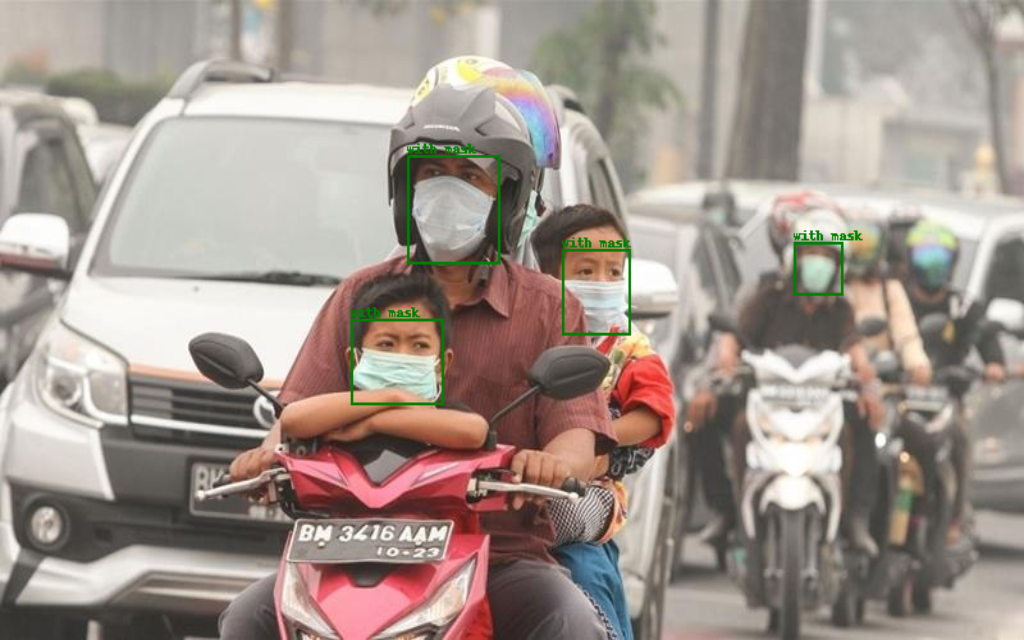
\includegraphics[width=\linewidth]{fig7e.png}
	\end{minipage}
	\begin{minipage}[t]{0.235\linewidth}
		\centering
		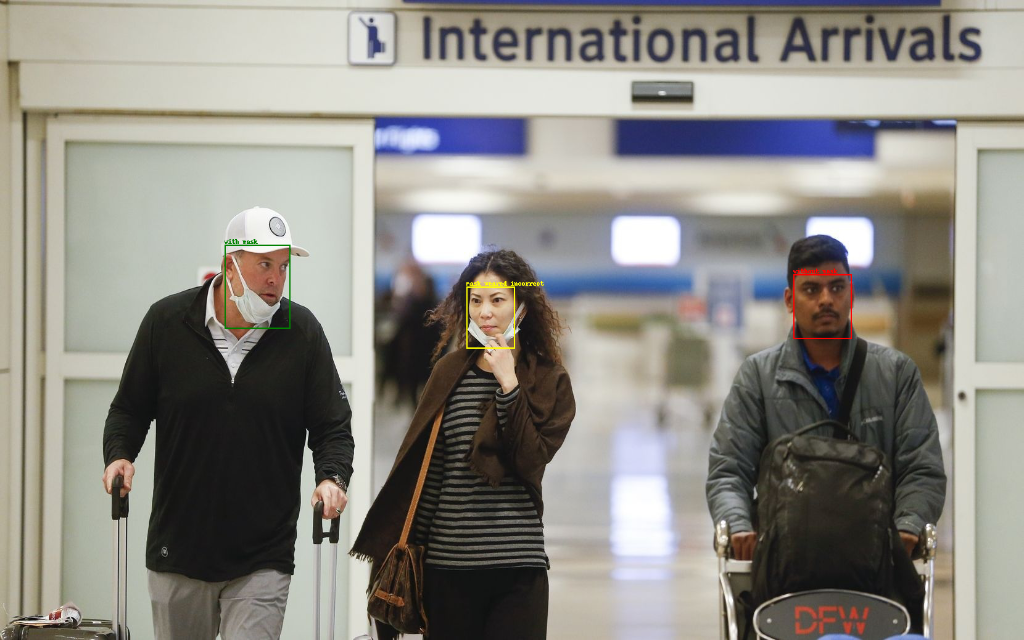
\includegraphics[width=\linewidth]{fig7b.png}\\
		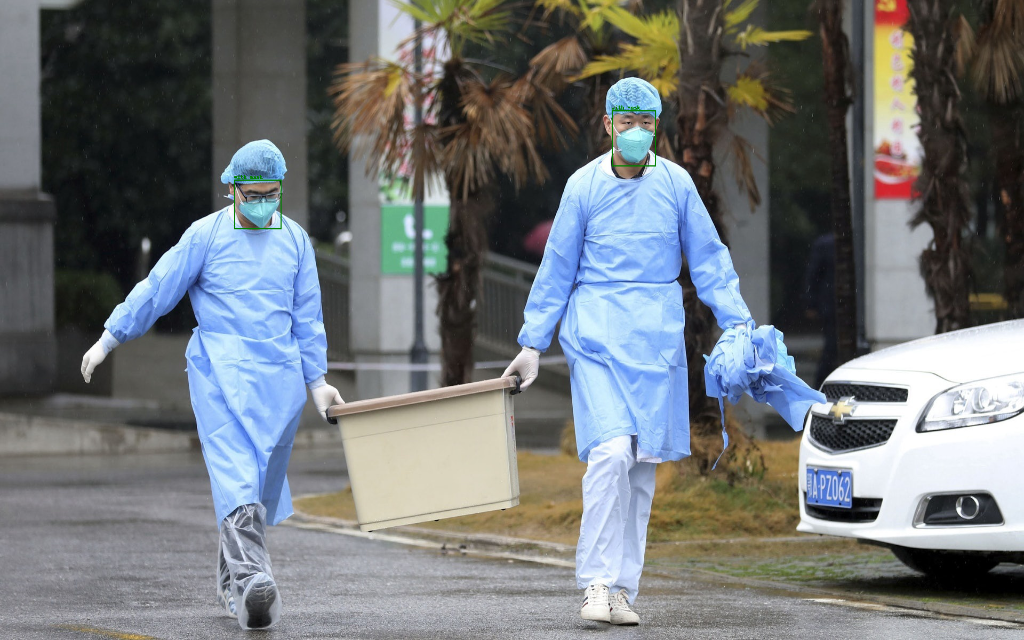
\includegraphics[width=\linewidth]{fig7f.png}
	\end{minipage}
	\begin{minipage}[t]{0.235\linewidth}
		\centering
		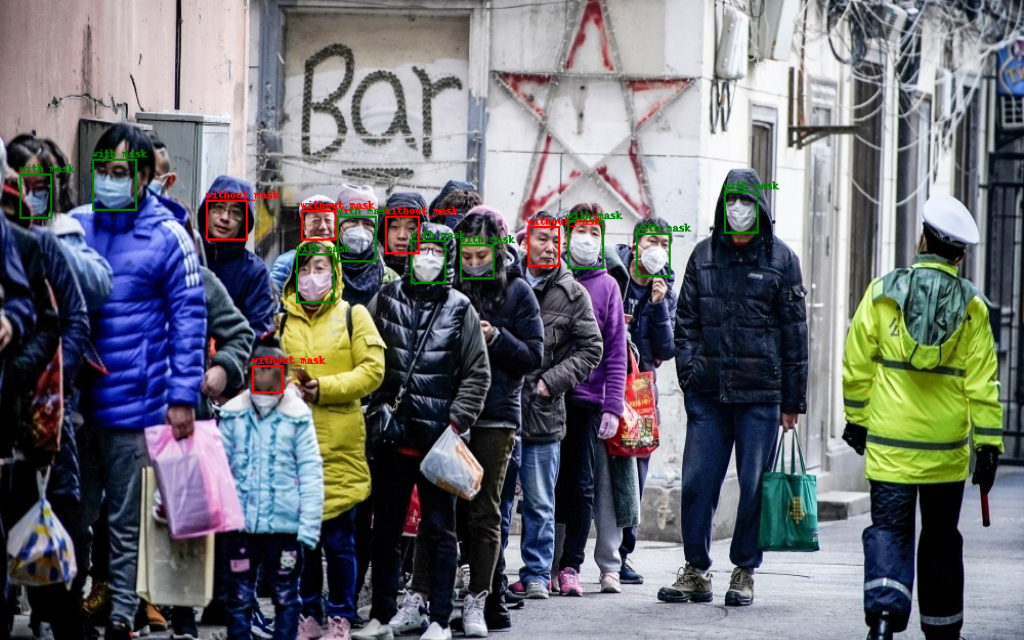
\includegraphics[width=\linewidth]{fig7c.png}\\
		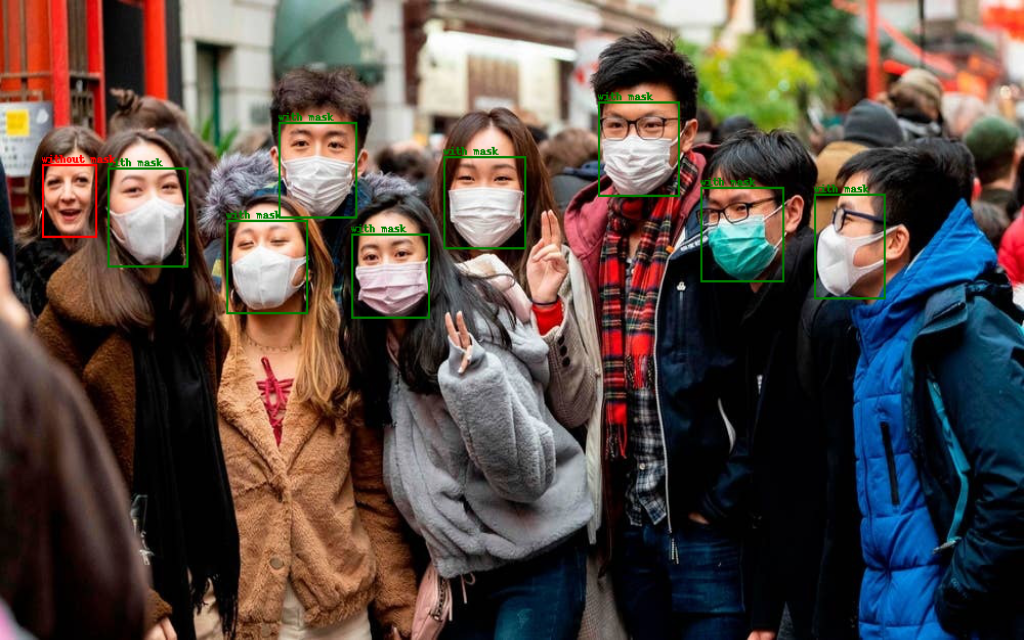
\includegraphics[width=\linewidth]{fig7g.png}
	\end{minipage}
	\begin{minipage}[t]{0.235\linewidth}
		\centering
		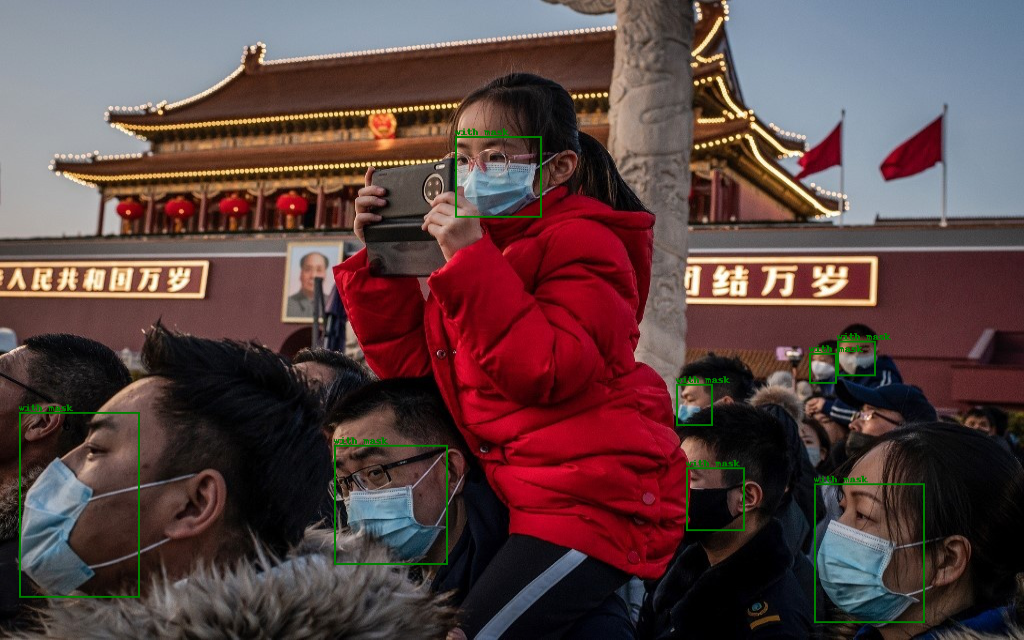
\includegraphics[width=\linewidth]{fig7d.png}\\
		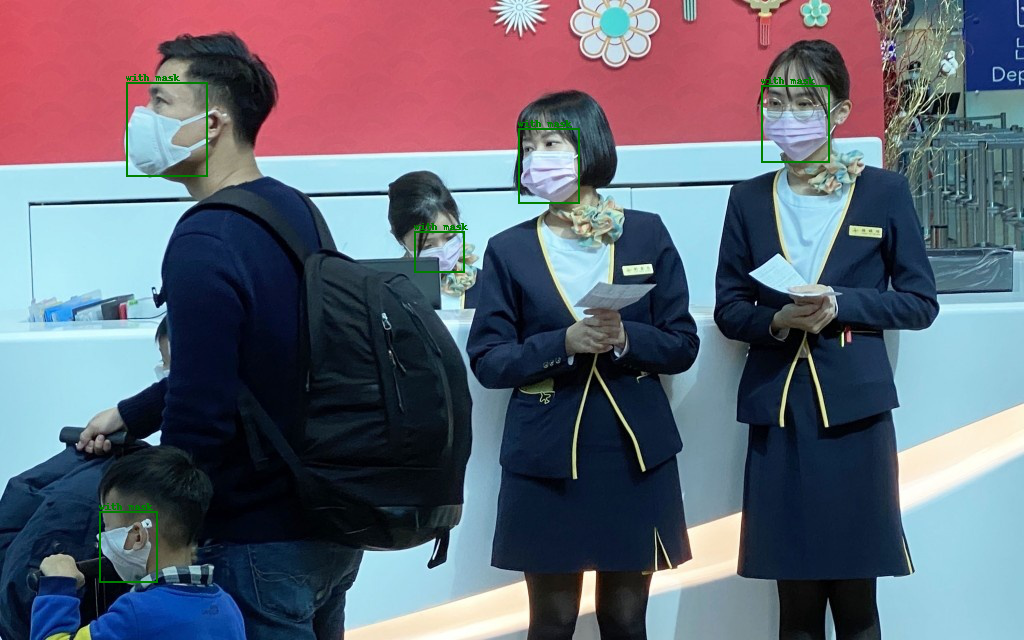
\includegraphics[width=\linewidth]{fig7h.png}
	\end{minipage}
	\caption{基于深度学习的口罩检测结果(部分)}
\label{fig:mask}
\end{figure}

\begin{table}[!ht]
	\centering
	\caption{基于深度学习的口罩检测评价指标}
	\begin{tabular}{c|c|cccc}
	\toprule
		&AP&AP$_{50}$&AP$_{75}$&AR$_1$&AR$_{10}$\\\hline
	Faster RCNN	&0.499&0.776&0.594&0.262&0.573\\
	\bottomrule
	\end{tabular}
	\label{tab:mask_metric}
\end{table}


实验在 PyTorch 提供的基于 COCO 数据集预训练的 Faster RCNN 模型调整预测器的输出类别后在 Mask Wearing 数据集上进行 finetune,训练 20--25 个 epoch 后验证集上的指标不在发生变化,在测试集上的评价指标如表 \ref{tab:mask_metric} 所示,检测结果如图 \ref{fig:mask} 所示。可以看到,深度学习模型可以对复杂场景进行较好的检测,如人群、侧脸或模糊的人脸,但同样由于样本邮箱,仍然会有检测失败的情形,如检测到不完整的人脸误判为未带口罩等。
